\documentclass{article}
%% \documentclass[pdftex]{article}
\usepackage[top=3cm,bottom=3cm,left=3.00cm,right=3.00cm]{geometry}
\usepackage{tikz,url}
\usepackage{xcolor}
\usepackage[colorlinks=true,urlcolor=blue,linkcolor=blue,citecolor=blue]{hyperref}
\usepackage{tkz-graph}
\usepackage{tikz}
\usetikzlibrary{positioning,chains,fit,shapes,calc}
%% \usetikzlibrary{graph}

\definecolor{processblue}{cmyk}{0.96,0,0,0}
\definecolor{myblue}{RGB}{80,80,160}
\definecolor{mygreen}{RGB}{80,160,80}

\newcounter{example}[section]
\newenvironment{example}[1][]{\refstepcounter{example}\par\medskip
  \begin{tabular}{|p{\textwidth}|}\hline\\{\bf EXAMPLE~\theexample. #1}}{\\\hline \end{tabular}}

\begin{document}

%% EX 1 %%%%%%%%%%%%%%%%%%%%%%%%%%%%%%%%%%%%%%%%%%%%
\begin{example}
  \begin{center}

    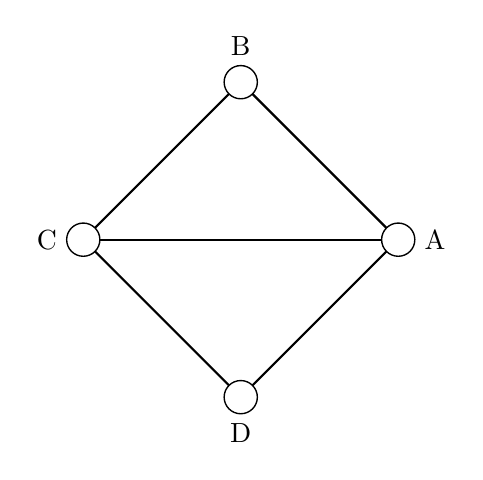
\begin{tikzpicture}
      \GraphInit[vstyle=Welsh]
      \SetGraphUnit{2}
      \Vertices{circle}{A,B,C,D}
      \Edges(A,B,C,D,A,C)
      \SetVertexNoLabel
    \end{tikzpicture}

  \end{center}

    {\small 
    \begin{verbatim}
    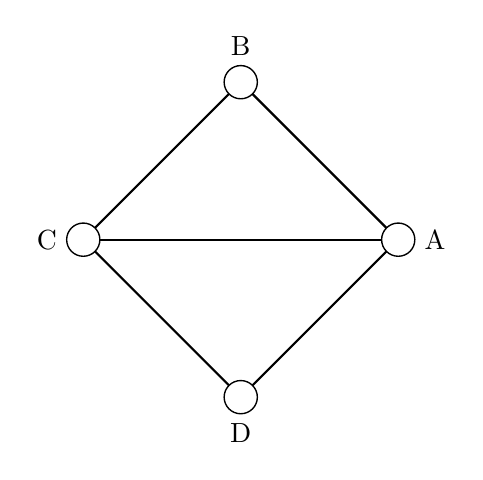
\begin{tikzpicture}
      \GraphInit[vstyle=Welsh]
      \SetGraphUnit{2}
      \Vertices{circle}{A,B,C,D}
      \Edges(A,B,C,D,A,C)
      \SetVertexNoLabel
    \end{tikzpicture}
    \end{verbatim}
    }

  
  source: \url{http://www.hoonzis.com/graph-theory-in-latex/}
\end{example}



%% EX 2 %%%%%%%%%%%%%%%%%%%%%%%%%%%%%%%%%%%%%%%%%%%%%%%%%%%%%%%%%
\begin{example}
  \begin{center}
    
    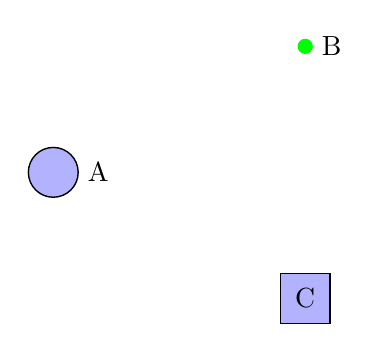
\begin{tikzpicture}[scale=0.8]
      % the next line  is because you want the style classic for most of the vertices
      % if you can't find a style in the predefined styles then you create a style with
      % \tikzset{VertexStyle/.style= ....
      % if a predefined style is not exactly what you want you can use after the next line
      % %\tikzset{VertexStyle/.append style = .....
      % You also use : \SetUpVertex  \SetUpVertex[FillColor=red] 
      %  \SetUpVertex is to avoid the use of \tikzset{VertexStyle/.append style ....   
      \GraphInit[vstyle=Classic]
      \SetUpVertex[FillColor=blue!30]  
      \Vertex{A}
      % with a scope you apply locally a new style but you can  use a tex group {....} instead.
      \begin{scope}[VertexStyle/.append style = {minimum size = 5pt, 
            inner sep = 0pt,
            color=green}]
        \Vertex[x=4,y=2]{B}   
      \end{scope}
      % here I use  \tikzset
      \tikzset{VertexStyle/.append style={rectangle}}
      % Now if I want to put the label inside the vertex, I need to pass the style in the  
      % options of Vertex with ,LabelOut=false.
      % Logically, it's possible with \SetUpVertex but ...
      \Vertex[x=4,y=-2,LabelOut=false]{C}  
    \end{tikzpicture}    
    %% ------------------------------------------------------
    \hskip5mm 
    %% ------------------------------------------------------
    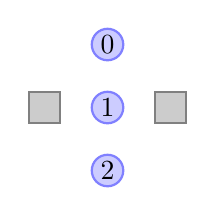
\begin{tikzpicture}[scale=0.8,
        place/.style={circle,draw=blue!50,fill=blue!20,thick,
          inner sep=0pt,minimum size=4mm},
        transition/.style={rectangle,draw=black!50,fill=black!20,thick,
          inner sep=0pt,minimum size=4mm}]
      \node at ( 0,2) [place] {0};
      \node at ( 0,1) [place] {1};
      \node at ( 0,0) [place] {2};
      \node at ( 1,1) [transition] {};
      \node at (-1,1) [transition] {};
    \end{tikzpicture}

  \end{center}
\end{example}

\bigskip


%% EX 3 %%%%%%%%%%%%%%%%%%%%%%%%%%%%%%%%%%%%%%%%%%%%%%%%%%%%%%%%%
\begin{example}
  \begin{center}
    
    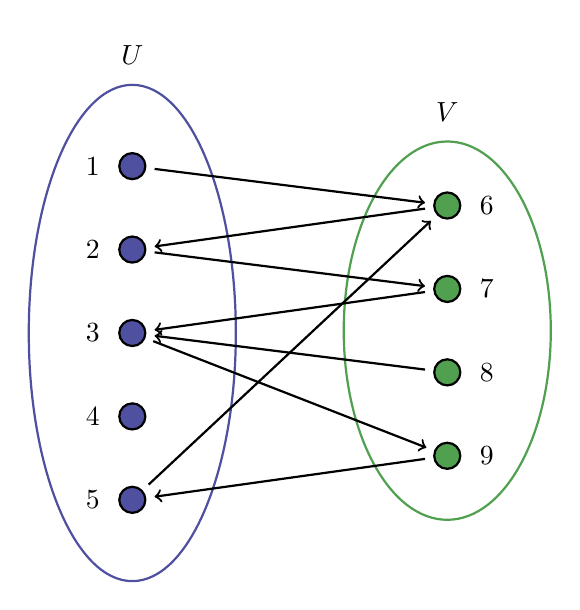
\begin{tikzpicture}[thick,
        every node/.style={draw,circle},
        fsnode/.style={fill=myblue},
        ssnode/.style={fill=mygreen},
        every fit/.style={ellipse,draw,inner sep=-2pt,text width=2cm},
        ->,shorten >= 3pt,shorten <= 3pt
      ]
      % the vertices of U
      \begin{scope}[start chain=going below,node distance=7mm]
        \foreach \i in {1,2,...,5}
        \node[fsnode,on chain] (f\i) [label=left: \i] {};
      \end{scope}

      % the vertices of V
      \begin{scope}[xshift=4cm,yshift=-0.5cm,start chain=going below,node distance=7mm]
        \foreach \i in {6,7,...,9}
        \node[ssnode,on chain] (s\i) [label=right: \i] {};
      \end{scope}

      % the set U
      \node [myblue,fit=(f1) (f5),label=above:$U$] {};
      % the set V
      \node [mygreen,fit=(s6) (s9),label=above:$V$] {};
      
      % the edges
      \draw (f1) -- (s6); \draw (s6) -- (f2); \draw (f2) -- (s7);
      \draw (s7) -- (f3); \draw (s8) -- (f3); \draw (f3) -- (s9);
      \draw (s9) -- (f5); \draw (f5) -- (s6);
 \end{tikzpicture}

  \end{center}

{\small 
\begin{verbatim}
      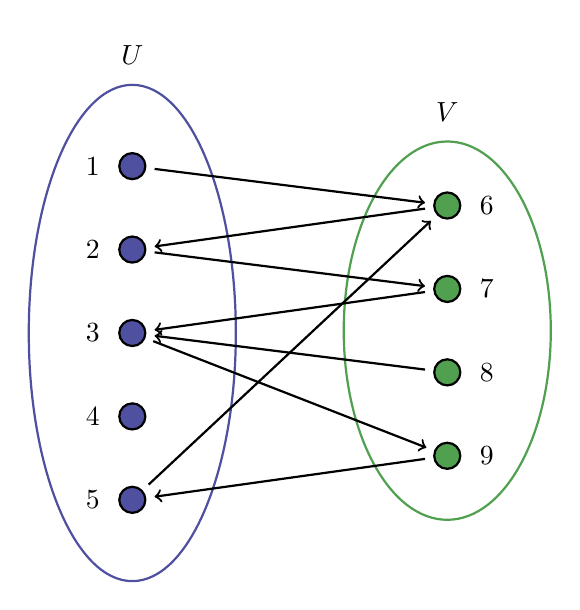
\begin{tikzpicture}[thick,
        every node/.style={draw,circle},
        fsnode/.style={fill=myblue},
        ssnode/.style={fill=mygreen},
        every fit/.style={ellipse,draw,inner sep=-2pt,text width=2cm},
        ->,shorten >= 3pt,shorten <= 3pt
      ]
      % the vertices of U
      \begin{scope}[start chain=going below,node distance=7mm]
        \foreach \i in {1,2,...,5}
        \node[fsnode,on chain] (f\i) [label=left: \i] {};
      \end{scope}

      % the vertices of V
      \begin{scope}[xshift=4cm,yshift=-0.5cm,start chain=going below,node distance=7mm]
        \foreach \i in {6,7,...,9}
        \node[ssnode,on chain] (s\i) [label=right: \i] {};
      \end{scope}

      % the set U
      \node [myblue,fit=(f1) (f5),label=above:$U$] {};
      % the set V
      \node [mygreen,fit=(s6) (s9),label=above:$V$] {};
      
      % the edges
      \draw (f1) -- (s6); \draw (s6) -- (f2); \draw (f2) -- (s7);
      \draw (s7) -- (f3); \draw (s8) -- (f3); \draw (f3) -- (s9);
      \draw (s9) -- (f5); \draw (f5) -- (s6); 
      \end{tikzpicture}
\end{verbatim}
}
  source \url{http://tex.stackexchange.com/questions/15088/bipartite-graphs}
\end{example}

\bigskip


%%  EX 4 %%%%%%%%%%%%%%%%%%%%%%%%%%%%%%%%%%%%%%%%%%%%%%%%%%%%%%%%%
\begin{example}
  \begin{center}

    \begin {tikzpicture}[
        -latex,auto,node distance =4 cm and 5cm,on grid,semithick,
        state/.style={circle,top color=white,bottom color=processblue!20,
          draw,processblue,text=blue,minimum width=1cm}
      ]
      \node[state] (C) {$1$};
      \node[state] (A) [above left=of C] {$0$};
      \node[state] (B) [above right =of C] {$2$};
      \path (A) edge [loop left] node[left] {$1/4$} (A);
      \path (C) edge [bend left =25] node[below =0.15 cm] {$1/2$} (A);
      \path (A) edge [bend right = -15] node[below =0.15 cm] {$1/2$} (C);
      \path (A) edge [bend left =25] node[above] {$1/4$} (B);
      \path (B) edge [bend left =15] node[below =0.15 cm] {$1/2$} (A);
      \path (C) edge [bend left =15] node[below =0.15 cm] {$1/2$} (B);
      \path (B) edge [bend right = -25] node[below =0.15 cm] {$1/2$} (C);
    \end{tikzpicture}

  \end{center}

    {\small 
    \begin{verbatim}
    \definecolor{processblue}{cmyk}{0.96,0,0,0}
    \begin {tikzpicture}[
        -latex,auto,node distance=4 cm and 5cm,on grid,semithick,
        state/.style={circle,top color=white,bottom color=processblue!20,
          draw,processblue,text=blue,minimum width=1cm}
      ]
      \node[state] (C) {$1$};
      \node[state] (A) [above left=of C] {$0$};
      \node[state] (B) [above right =of C] {$2$};
      \path (A) edge [loop left] node[left] {$1/4$} (A);
      \path (C) edge [bend left =25] node[below =0.15 cm] {$1/2$} (A);
      \path (A) edge [bend right = -15] node[below =0.15 cm] {$1/2$} (C);
      \path (A) edge [bend left =25] node[above] {$1/4$} (B);
      \path (B) edge [bend left =15] node[below =0.15 cm] {$1/2$} (A);
      \path (C) edge [bend left =15] node[below =0.15 cm] {$1/2$} (B);
      \path (B) edge [bend right = -25] node[below =0.15 cm] {$1/2$} (C);
    \end{tikzpicture}
    \end{verbatim}
    }

  source \url{http://www.guitex.org/home/images/doc/GuideGuIT/introingtikz.pdf}
\end{example}

\bigskip



%% EX 5 %%%%%%%%%%%%%%%%%%%%%%%%%%%%%%%%%%%%%%%%%%%%%%%%
\begin{example}
  \begin{center}

    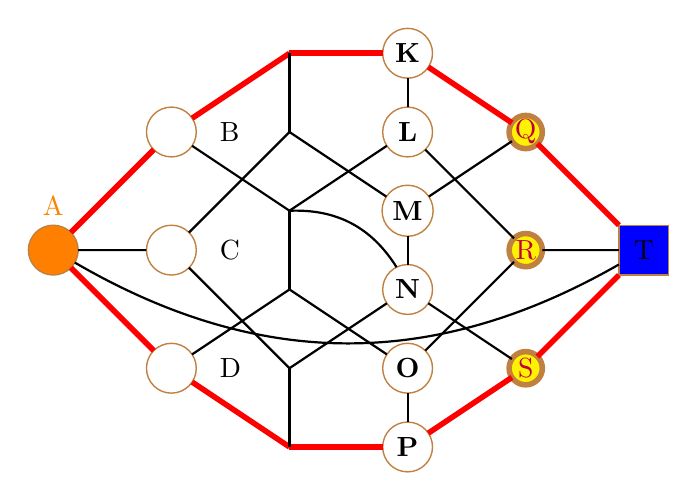
\begin{tikzpicture}
      \SetVertexNormal[LineColor=brown]
          {\renewcommand{\VertexLightFillColor}{orange}\Vertex[x=0,y=2.5,style=orange,LabelOut=true,Lpos=90]{A}}
          {\SetGraphUnit{1.5}\Vertices[x=1.5,y=4,dir=\SO,LabelOut=true,Ldist=5pt]{line}{B,C,D}}
          {\renewcommand{\VertexShape}{coordinate}\Vertices[x=3,y=5,dir=\SO]{line}{E,F,G,H,I,J}}
          \Vertices[x=4.5,y=5,dir=\SO,style={font=\bfseries}]{line}{K,L,M,N,O,P}
          {\SetGraphUnit{1.5}
            \renewcommand{\VertexLineWidth}{2pt}
            \renewcommand{\VertexInnerSep}{0pt}
            \renewcommand{\VertexTextColor}{purple}
            \renewcommand{\VertexLightFillColor}{yellow}
            \renewcommand{\VertexInterMinSize}{12pt}
            \Vertices[x=6,y=4,dir=\SO]{line}{Q,R,S}}
          {\renewcommand{\VertexShape}{rectangle}\renewcommand{\VertexLightFillColor}{blue}\Vertex[x=7.5,y=2.5]{T}}
          \Edges[local,color=red,lw=2pt](A,B,E,K,Q,T,S,P,J,D,A)
          \Edges(B,G,L,R,T)
          \Edges(D,H,O,R)
          \Edges(A,C,F,M,Q)
          \Edges(C,I,N,S)
          \foreach \x/\y in {E/F,G/H,I/J,K/L,M/N,O/P}
                   {\Edge(\x)(\y)}
                   \Edge[style={bend left}](G)(N)
                   \Edge[style={bend right}](A)(T)
    \end{tikzpicture}

  \end{center}
  
  source: \url{https://graphtheoryinlatex.wordpress.com/}
\end{example}


\bigskip


%% EX 6 %%%%%%%%%%%%%%%%%%%%%%%%%%%%%%%%%%%%%%%%%%%%%%%%
\begin{example}
  \begin{center}

    \tikzstyle{roundnode} = [circle, draw=green!60, fill=green!5, very thick, minimum size=7mm]
    \tikzstyle{squarednode} = [rectangle, draw=red!60, fill=red!5, very thick, minimum size=5mm]

    \begin{tikzpicture}[scale=1.2]
      %Nodes
      \node[squarednode]      (maintopic)                              {2};
      \node[roundnode]        (uppercircle)       [above=of maintopic] {1};
      \node[squarednode]      (rightsquare)       [right=of maintopic] {3};
      \node[roundnode]        (lowercircle)       [below=of maintopic] {4};
 
      %Lines
      \draw[->] (uppercircle.south) -- (maintopic.north);
      \draw[->] (maintopic.east) -- (rightsquare.west);
      \draw[->] (rightsquare.south) .. controls +(down:7mm) and +(right:7mm) .. (lowercircle.east);
    \end{tikzpicture}
  \end{center}
\end{example}

\bigskip


%% EX 7 %%%%%%%%%%%%%%%%%%%%%%%%%%%%%%%%%%%%%%%%%%%%%%%%
\begin{example}
  \begin{center}
    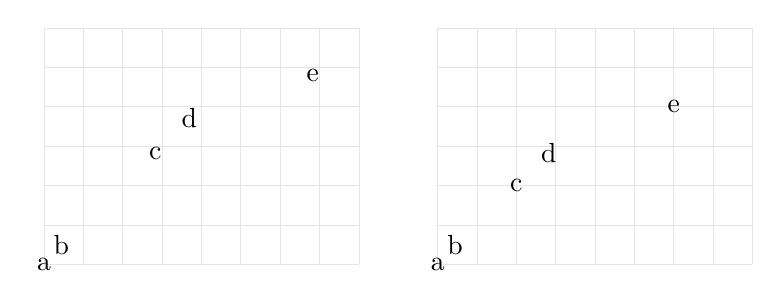
\begin{tikzpicture}  
      \draw[help lines,step=5mm,gray!20] (0,0) grid (4,3);
      \node (a) at (0,0) {a};  
      \node[above right] (b) {b};
      \node[above right = of a] (c) {c};
      \node[above right = 2cm of a] (d) {d};
      \node[above right = 2cm and 3cm of a] (e) {e};
      \begin{scope}[xshift=5cm,on grid]
        \draw[help lines,step=5mm,gray!20] (0,0) grid (4,3);
        \node (a) at (0,0) {a};  
        \node[above right] (b) {b};
        \node[above right = of a] (c) {c};
        \node[above right = 2cm of a] (d) {d};
        \node[above right = 2cm and 3cm of a] (e) {e};
      \end{scope}
    \end{tikzpicture} 
  \end{center}
\end{example}

\bigskip

%% EX 8 %%%%%%%%%%%%%%%%%%%%%%%%%%%%%%%%%%%%%%%%%%%%%%%%
\begin{example}
    Hello \tikz [baseline] \fill [fill=blue!80!black] (0,.75ex) circle[radius=.75ex];

  source: pgfmanual (page 115)\\
  \url{http://ctan.sharelatex.com/tex-archive/graphics/pgf/base/doc/pgfmanual.pdf#page=41}

\end{example}

\newpage

%% EX 9 %%%%%%%%%%%%%%%%%%%%%%%%%%%%%%%%%%%%%%%%%%%%%%%%
\begin{example}
  \begin{center}
    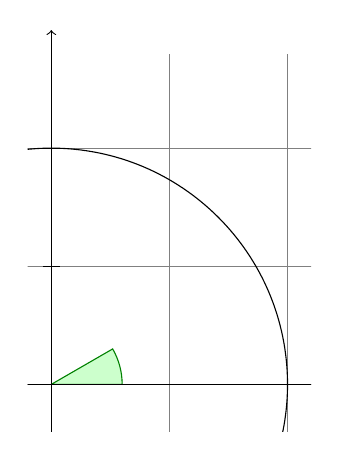
\begin{tikzpicture}[scale=3]
      \clip (-0.1,-0.2) rectangle (1.1,1.51);
      \draw[step=.5cm,gray,very thin] (-1.4,-1.4) grid (1.4,1.4);
      \filldraw[fill=green!20,draw=green!50!black] (0,0) -- (3mm,0mm)
      arc [start angle=0, end angle=30, radius=3mm] -- cycle;
      \draw[->] (-1.5,0) -- (1.5,0);
      \draw[->] (0,-1.5) -- (0,1.5);
      \draw (0,0) circle [radius=1cm];
      \foreach \x in {-1cm,-0.5cm,1cm}
      \draw (\x,-1pt) -- (\x,1pt);
      \foreach \y in {-1cm,-0.5cm,0.5cm,1cm}
      \draw (-1pt,\y) -- (1pt,\y);
    \end{tikzpicture}

    \bigskip

    \begin{tikzpicture}[scale=3]
      \foreach \x in {-1,-0.5,1} 
      \draw[xshift=\x cm] (0pt,-1pt) -- (0pt,1pt);
    \end{tikzpicture}

  \end{center}
    source: pgfmanual (page 41)
    %% http://ctan.sharelatex.com/tex-archive/graphics/pgf/base/doc/pgfmanual.pdf#page=41

\end{example}

\bigskip

%% EX 10 %%%%%%%%%%%%%%%%%%%%%%%%%%%%%%%%%%%%%%%%%%%%%%%%
% Drawing a graph
% Author: Stefan Kottwitz
% https://www.packtpub.com/hardware-and-creative/latex-cookbook
\begin{example}
  \begin{center}
    \GraphInit[vstyle = Shade]
    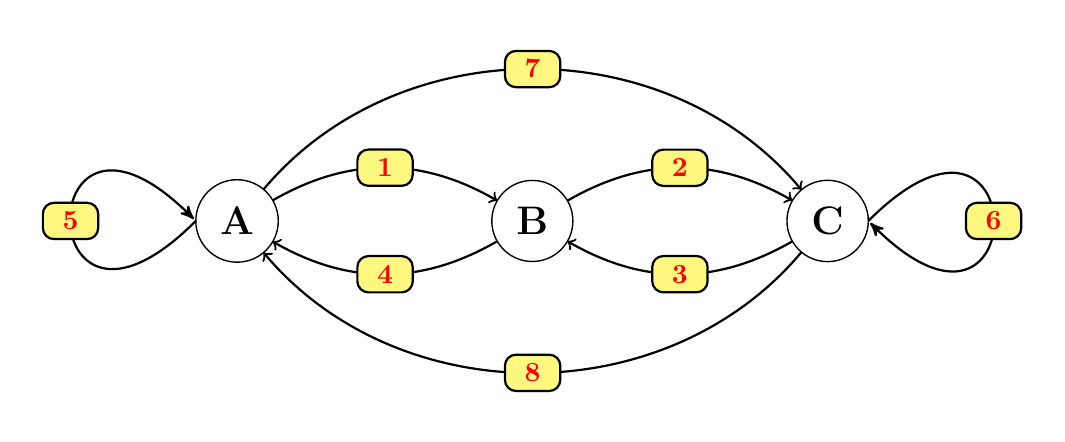
\begin{tikzpicture}[scale=.75,
        LabelStyle/.style = { rectangle, rounded corners, draw,
          minimum width = 2em, fill = yellow!50,
          text = red, font = \bfseries },
        VertexStyle/.append style = { inner sep=5pt,
          font = \Large\bfseries},
        EdgeStyle/.append style = {->, bend left} 
      ]
      \SetGraphUnit{5}
      \Vertex{B}
      \WE(B){A}
      \EA(B){C}
      \Edge[label = 1](A)(B)
      \Edge[label = 2](B)(C)
      \Edge[label = 3](C)(B)
      \Edge[label = 4](B)(A)
      \Loop[dist = 4cm, dir = NO, label = 5](A.west)
      \Loop[dist = 4cm, dir = SO, label = 6](C.east)
      \tikzset{EdgeStyle/.append style = {bend left = 50}}
      \Edge[label = 7](A)(C)
      \Edge[label = 8](C)(A)
    \end{tikzpicture}
  \end{center}
\end{example}

\newpage



%% EX 11 %%%%%%%%%%%%%%%%%%%%%%%%%%%%%%%%%%%%%%%%%%%%%%%%
% finite state automata (fsa)
\begin{example}
  \begin{center}
    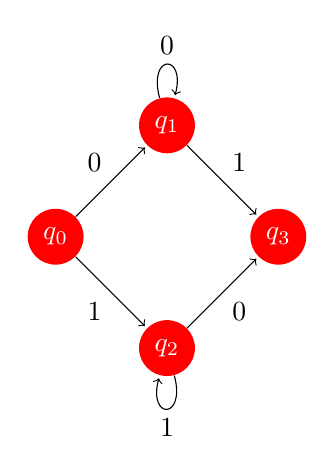
\begin{tikzpicture}[shorten >=1pt,node distance=2cm,on grid,auto,
        state/.style={fill=red,draw=none,circle,text=white}]
      %% \draw[help lines] (0,0) grid (3,2);
      \node[state] (q_0) {$q_0$};
      \node[state] (q_1) [above right=of q_0] {$q_1$};
      \node[state] (q_2) [below right=of q_0] {$q_2$};
      %% \node[state,accepting](q_3) [below right=of q_1] {$q_3$};
      \node[state](q_3) [below right=of q_1] {$q_3$};
      \path[->] (q_0) edge node {0} (q_1)
      edge node [swap] {1} (q_2)
      (q_1) edge node {1} (q_3)
      edge [loop above] node {0} ()
      (q_2) edge node [swap] {0} (q_3)
      edge [loop below] node {1} ();
    \end{tikzpicture}
  \end{center}
\end{example}

\bigskip

%% EX 12 %%%%%%%%%%%%%%%%%%%%%%%%%%%%%%%%%%%%%%%%%%%%%%%%
% finite state automata (fsa)
\begin{example}
  \begin{center}
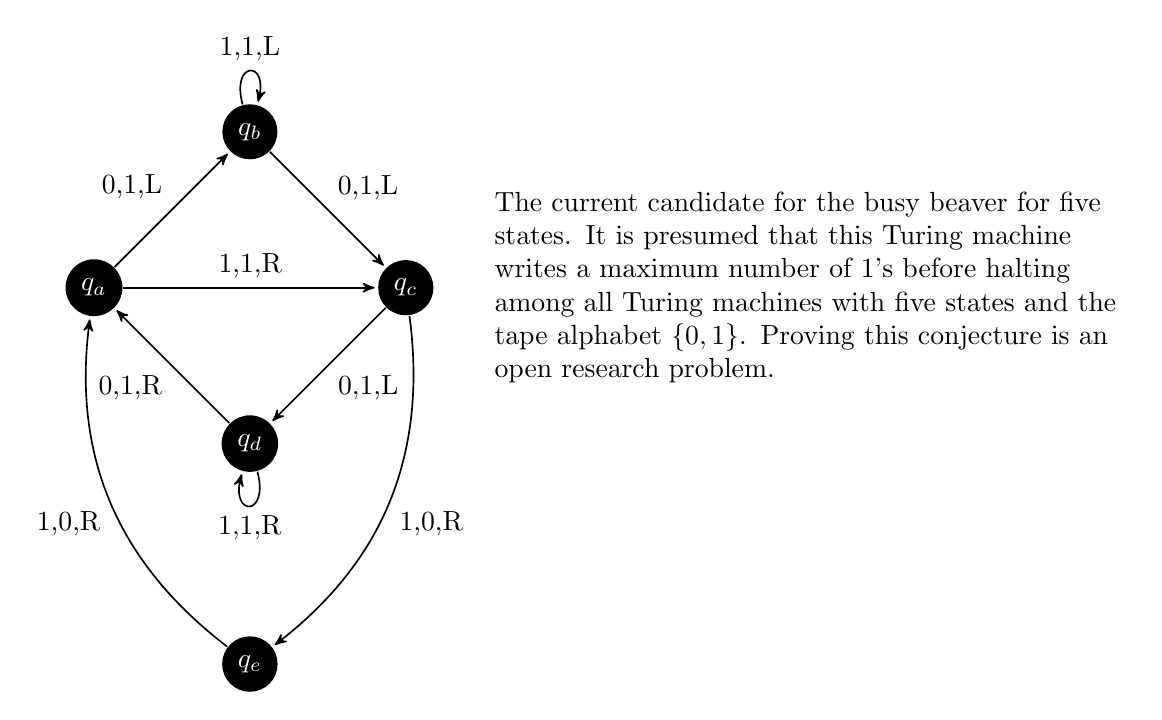
\begin{tikzpicture}[
    ->,>=stealth',shorten >=1pt,
    auto,node distance=2.8cm,on grid,semithick,
    state/.style={fill=black,draw=none,circle,text=white}
  ]
  \node[state] (A) {$q_a$};
  \node[state] (B) [above right=of A] {$q_b$};
  \node[state] (D) [below right=of A] {$q_d$};
  \node[state] (C) [below right=of B] {$q_c$};
  \node[state] (E) [below=of D] {$q_e$};
  \path (A) edge node {0,1,L} (B)
  edge node {1,1,R} (C)
  (B) edge [loop above] node {1,1,L} (B)
  edge node {0,1,L} (C)
  (C) edge node {0,1,L} (D)
  edge [bend left] node {1,0,R} (E)
  (D) edge [loop below] node {1,1,R} (D)
  edge node {0,1,R} (A)
  (E) edge [bend left] node {1,0,R} (A);
  \node [right=1cm,text width=8cm] at (C)
        {
          The current candidate for the busy beaver for five states. It is
          presumed that this Turing machine writes a maximum number of
          $1$’s before halting among all Turing machines with five states
          and the tape alphabet $\{0, 1\}$. Proving this conjecture is an
          open research problem.
        };
\end{tikzpicture}

  \end{center}
\end{example}

\newpage


%% EX 13 %%%%%%%%%%%%%%%%%%%%%%%%%%%%%%%%%%%%%%%%%%%%%%%%
% cyclic graphs
\begin{example}
  \begin{center}

    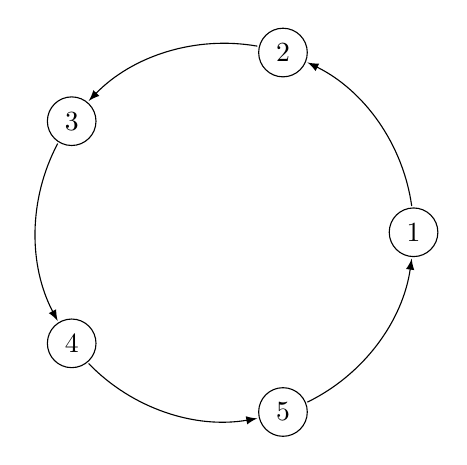
\begin{tikzpicture}[scale=0.8]
      \def \n {5}
      \def \radius {3cm}
      \def \margin {8} % margin in angles, depends on the radius
      \foreach \s in {1,...,\n}
               {
                 \node[draw, circle] at ({360/\n * (\s - 1)}:\radius) {$\s$};
                 \draw[->, >=latex] ({360/\n * (\s - 1)+\margin}:\radius) 
                 arc ({360/\n * (\s - 1)+\margin}:{360/\n * (\s)-\margin}:\radius);
               }
    \end{tikzpicture}
    %% ------------------------------------------------------
    \hskip5mm 
    %% ------------------------------------------------------
    \begin{tikzpicture}
      \def \n {4}
      \def \m {3}
      \def \radius {3cm}
      \def \margin {8} % margin in angles, depends on the radius
      \foreach \s in {0,...,\m}
               {
                 \node[draw, circle] at ({360/\n * (\s)}:\radius) {$\s$};
                 \draw[->, >=latex] ({360/\n * (\s)+\margin}:\radius) 
                 arc ({360/\n * (\s)+\margin}:{360/\n * (\s+1)-\margin}:\radius);
               }
    \end{tikzpicture}

  \end{center}

\end{example}


\end{document}
